\chapter{State of the art}

% \section{Intraoperative ultrasound}
% \textcolor{green}{Start with why US is used, then describe how it works and the limitations. from there you should have a nice transition to navigation}
% In
% liver surgeries an intraoperative ultrasound device is used for intraoperative planning and
% navigation inside the liver. It is used to locate tumors that are not
% visible on the liver surface and to estimate their sizes from the ultrasound image. Figure \ref{fig:liverUS} shows an example of an
% ultrasound image of the liver and its corresponding position in the 3D liver
% model.

% \begin{figure}[H]
%   \centering
%  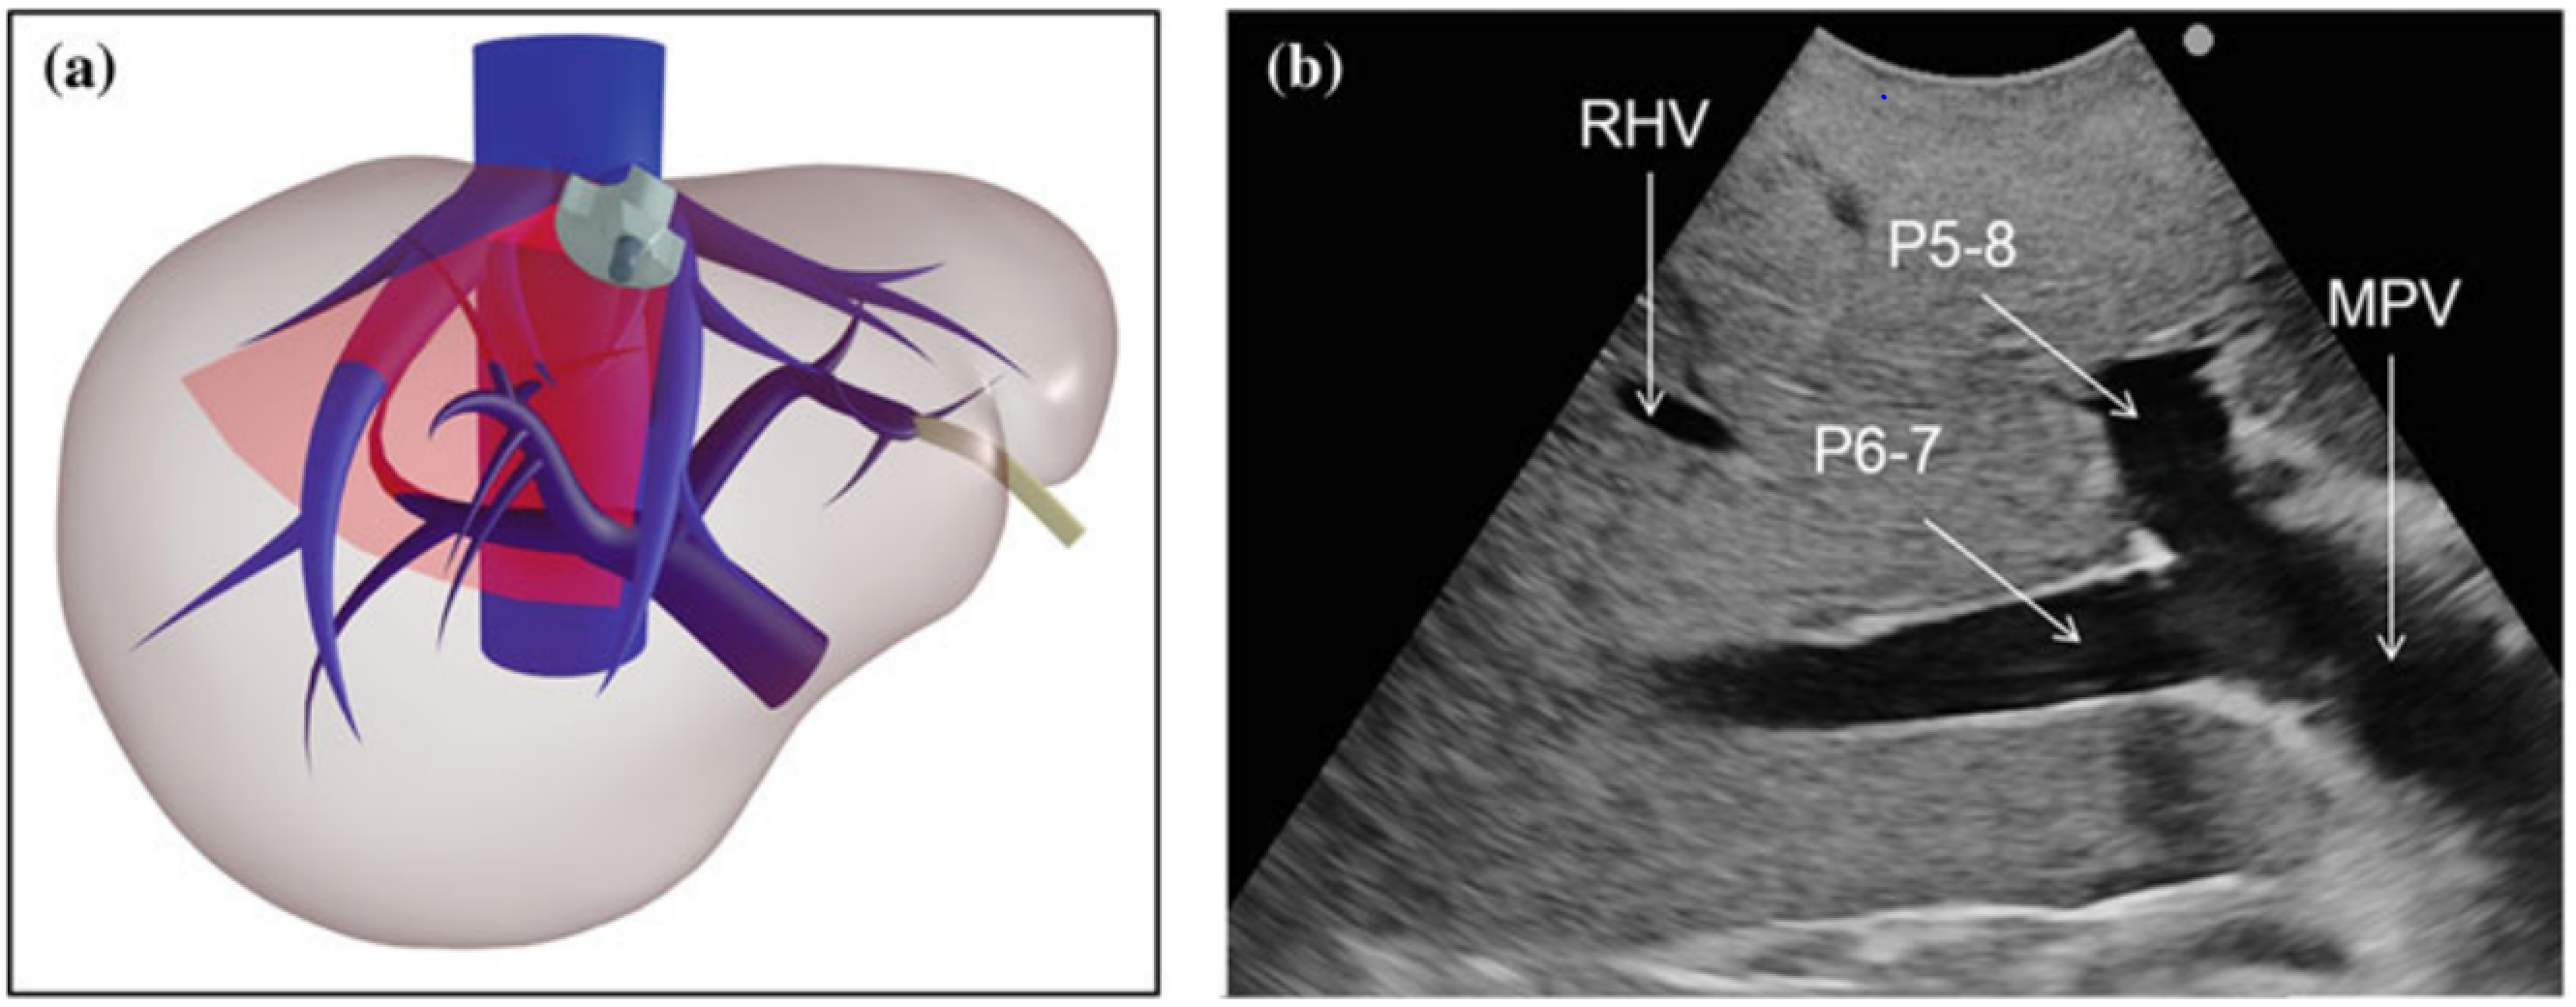
\includegraphics[width=\textwidth]{liverUS}
%  \caption{ Left (a) ultrasound image plane in the liver. Right (b) intraoperative
%    ultrasound image. One can see the right hepatic vein (RHV), the portal branch
%    to segments 5 and 8 (P5-8) and the portal branch to segments 6 and 7 (P6-7) \cite{torzilli2014ultrasound}}
%   \label{fig:liverUS}
% \end{figure}

% Ultrasound imaging works by the \textit{pulse-echo} principle. A short
% ultrasound pulse is emitted from a transducer. The sound waves get
% transmitted and reflected differently by different tissues. The reflected
%  waves travel back into the transducer and are converted into an electrical
% signal. After post-processing these signals become ultrasound images. 
% The ultrasound measures the mechanical properties of the tissue. The tissues
% have different acoustic impedance, which is the product of tissue density and
% ultrasound speed in travelling through the tissue. The resolution of the
% ultrasound images depends on the frequency of the ultrasonic waves. High
% frequencies lead to higher resolution but lower penetration depth into the tissue because the
% absorption of the sound energy increases with frequency too. Therefore the
% useability to see deep structures is limited \cite{torzilli2014ultrasound}. 

% In liver surgeries ultrasound is an important and established instrument.
% Intraoperatively, the ultrasound is used on the liver surface directly,
% therefore the penetration depth of the
% ultrasound is optimal to represent the inner structures of the liver.
% Registration methods based on 3D ultrasound reconstructed liver vessels 
% exist but are not used in practice frequently \cite{lange2003vessel}. Ultrasound
% is not harmful to health and therefore, can
% be used as often as desired to navigate during a surgery.
% % it is  
% % Intraoperatively surgeons use ultrasound to localize the tumor as it gives
% % advantages of reduced surgical time, complexity and radiation dosage.

% \section{Navigation for liver resections}
% \label{sec:navigationForLiverResections}
% \textcolor{green}{first, why is navigation needed, then how does it generally work
%   1) preoperative model or surgical plan 2) tracking 3) registration 4)
%   navigation visualization etc. then challenges especially in liver surgery and limitations}
% It is a difficult task for inexperienced surgeons to orientate themselves within the liver during an operation.
% From the outside of the liver it is not visible where the blood vessels are which they do not want to hurt.
% Navigation can help surgeons to orient themselves precisely in organs during
% operations.

% % The actual intervention in computer assisted surgeries (CAS) is defined as
% % surgical navigation.
% A navigated operation differs in a few points from a non-navigated operation.
% Because every patient's liver is different, a new 3D model of the liver has to
% be created before surgery. This models are created from pre-operative 3D
% computer tomography (CT) scan of the liver. Then, using this model, a surgical plan is made.
% In contrast to a regular operation, a navigation system is located in the
% operating theatre and the surgical instruments can be tracked by it. Therefore special instruments are used. These
% instruments have the ability to be tracked by the naviagation system. Depending
% on the tracking technology used by the navigation system, the tools are different.
% In order to also track the liver, the created model is registered to the anatomy
% of the patient. Finally the orientation and position
% of the instruments in relation to the patient's anatomy is visualized on a
% monitor in the operating room. The surgeon can see what he does on the
% monitor and uses the system to navigate the location and position of its
% instruments. This is specialy then useful when the tip of the instrument is not
% actually visible for the suergeon.

% The achieved
% navigation accuracy with such a system was 4.5 mm $\pm$3.6 mm averaged over nine surgeries \cite{peterhans2011navigation}.
% Current research tries to compensate for deformations of the liver after the CT
% scan to the actual shape of the liver \cite{clements2017deformation}
% \cite{clements2015validation}. 
% \subsection{Creation of preoperative 3D-models}
% Several steps are necessary to create a preoperative model. First the 
% CT scan is done. This leads to representations of the liver on several 2D images parallel
% to each other, filling a square volume with voxels. From this data the liver and
% its inner structures are manually segmented and merged to a 3D model (Figure \ref{fig:MeVisExample}). This is very
% time consuming and therefore expensive \cite{numminen2005preoperative}.
% Nevertheless the resulting models are very detailed and accurate.
% \begin{figure}[H]
%   \centering
%  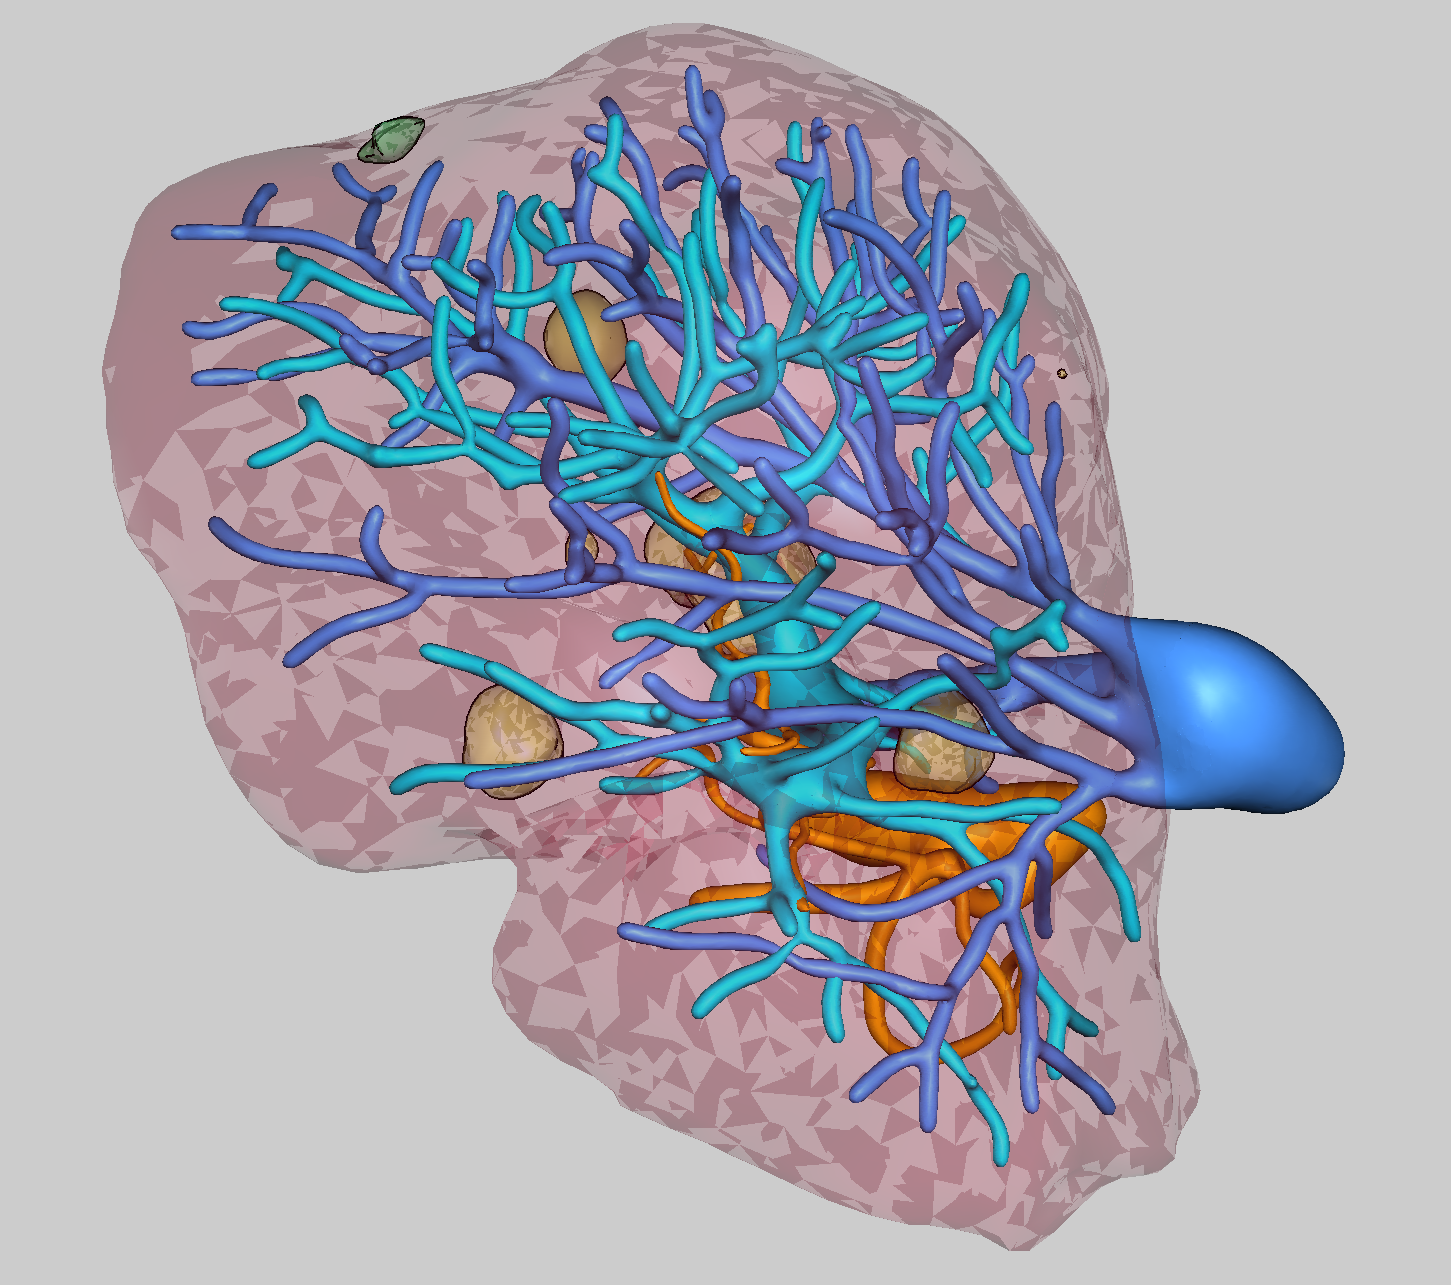
\includegraphics[width=0.6\textwidth]{MeVisExample}
%  \caption{Example of a preoperative 3D model created by MeVis}%DK patient
%   \label{fig:MeVisExample}
% \end{figure}

% \subsection{Registration methods}
% Patient registration is a concept to correlate the reference coordinate system
% of a virtual 3D data set with that of a patient. First, the 3D data set has to
% be gathered. This is often done by CT or MRI scan of the patients anatomy to be
% operated on. Secondly, finding of the transformation between the patient's
% reference coordinate system and the virtual data set. During the surgery the patient is similarly
% tracked as the instruments (see section \ref{sec:navigationForLiverResections}).
% In this way, the patient has his own coordinate system. From here many different
% methods exist to align the virtal data to the real anatomy.
% Discrete landmarks, surface scans and
% volumetric sonography scans are just a few of the approaches that can be
% used to achieve precise alignment of the data with the
% surgical site \cite{banz2016intraoperative}. 

% \subsubsection{Surface registration}
% Surface registration is registration based on surfaces. It is used and studied
% for several years in all kinds of fields \cite{ramos2015review}. Especially in
% the field of medical technology, a lot of research is being done in the
% direction of contactless registration. Intraoperatively, different camera technologies which lead
% to depth images are used to sample the surface of an organ. Often used imaging systems are stereo cameras
% \cite{furukawa2010accurate}, structured light \cite{salvi2004pattern} and
% laser range scanners \cite{cash2003incorporation}. From these intraoperatively
% created data sets, surfaces are reconstructed and then used for registration. To
% find the mapping between the surfaces, mostly different variants of the iterative
% closest point (ICP) \cite{besl1992method} algorithm are used. 

% These surface based methods are limited for different reasons. In most cases
% only part of the whole organ can be seen (scanned). The scanned surface may lack
% of unique structures on the surface. The scanning process can 
% lead to noisy data. The organ of interest may be deformed between the
% acquisitions of the surface samples. Therefore researchers try to compensate for
% intraoperative soft-tissue deformations \cite{cash2005compensating}\cite{dagon2008real}.
% \subsection{Tracking modalities}
% To track surgical instruments and patient's anatomy (define the position and
% orientation in real time) during naviagated surgery a tracking system is needed.
% Tracking can be done by different technologies. The most used tracking
% modality is optical tracking. 

% \subsubsection{Optical tracking}
% Optical tracking is the most used tracking modality in naviagated liver
% surgeries. Passive markers (spherical, retro-reflective that reflect infrared
% light) or active markers (infrared-emitting markers that are activated by an
% electrical signal) \cite{wiles2004accuracy} are attached to the objects that
% need to be tracked. A tracking camera is then emitting infrared light by illuminators
% on the position sensor (only for passive markers). The position sensor
% determines the position and orientation of the tracked instruments based on the
% information it receives from those markers \cite{noauthor_polaris_nodate}.  
\section{Ultrasound based registration}
\section{Creating models from intraoperative imaging for liver resection surgeries}
\section{Deficits of existing solutions}
\section{Objectives} 
The objectives of this Master's thesis are:
\begin{itemize}
  \item Implementation of the concept for an intraoperative 3D reconstrction
  technique of the liver from intraoperative ultrasound. 
  \item Implementation of the intraoperative resection planning.
\end{itemize}
This work focuses on open surgical procedures of liver hepatectomies and
especially parenchymal-sparing methods.





% \begin{itemize}
%   \item not tracked laproscopic one shot images stereo with registration
%   \item moved laproscopic tracked endoscope stereo with registration 
% \end{list}

% \cite{hoppe1992surface}

\endinput
%%% Local Variables:
%%% TeX-master: "MscThesis"
%%% End: